\documentclass{article}
\usepackage[utf8]{inputenc}
\usepackage[margin=1 in]{geometry}
\usepackage{graphicx}
\usepackage[colorlinks]{hyperref}
\usepackage{listings}
\usepackage{color}
\usepackage{algorithm}
\usepackage{algorithmic}
\usepackage{float} %for floating images
\usepackage[table,xcdraw]{xcolor} %for colored tables

\hypersetup{
  colorlinks=true,
  urlcolor=blue
}

\definecolor{dkgreen}{rgb}{0,0.6,0}
\definecolor{gray}{rgb}{0.5,0.5,0.5}
\definecolor{mauve}{rgb}{0.58,0,0.82}

\lstset{frame=tb,
  language=Python,
  aboveskip=3mm,
  belowskip=3mm,
  showstringspaces=false,
  columns=flexible,
  basicstyle={\small\ttfamily},
  numbers=left,
  numberstyle=\tiny\color{gray},
  keywordstyle=\color{blue},
  commentstyle=\color{dkgreen},
  stringstyle=\color{mauve},
  breaklines=true,
  breakatwhitespace=true,
  tabsize=3
}


\author{Matheus Augusto da Silva - Alessandro Montaldo}
\title{\textbf{SR2I 203 - État de l'art, études initiaux}}
\date{\today}

\begin{document}
\maketitle

%--------------------------
\section{Introduction}
Notre projet consiste en l’étude et la mise en œuvre d’un type spécifique d’attaque par déni de service, une
Attaque de type Low et Slow, l’attaque Slowloris. L’objectif de ce rapport est de présenter les études et les progrès réalisés et d’expliquer et de motiver les
seront nos prochaines étapes. En particulier nous avons suivi le chemin: \\

\begin{itemize}
	\item une étude concentrée sur la compréhension des fonctionnalités principales du protocole HTTP et du serveur Web Apache.
	\item une recherche concentrée sur l'attaque de slowloris.
	\item a realisation of a first implementation in Python using the software Scapy of the basic functionallity of the attack.
\end{itemize}

%\noindent
%The next step to be accomplished are finally listed. \\
%Next steps are then explained in the last section. 

%--------------------------
\section{Étude du Protocole HTTP}
Hypertext Transfer Protocol a été conçu avec le but de construire une architecture client-serveur tel qu'on peut implémenter un déploiement du WWW. C'est un protocole de la couche application et il permet l'implémentation d'un des outils les plus populaires d'Internet aujourd'hui: le navigateur Web. \\
Le principe c'est d'une architecture où un site web (serveur ou ensemble de serveurs) est associé à plusieurs ressources lesquelles un client peut demander via les méthodes HTTP. Un serveur web peut être identifié par son URL ou son adresse IP et généralement garde informations comme pages web, images et fichiers.

\subsection{HTTP Requests and responses}
Each request begins with a Request-Line that indicates specific method, the resource to which the method applies, and the version of http that the client can support. One or more message headers can follow and a message body separated with a blank line. \\

\noindent
HTTP responses look a lot like HTTP requests. The only significant difference is that responses begin with a status line rather than a Request-Line.

\begin{figure}[H]
	\begin{center}
		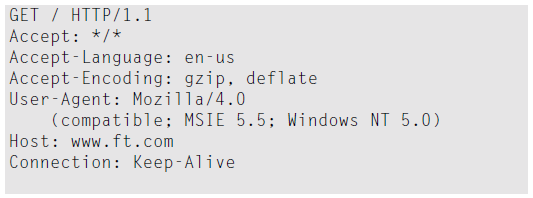
\includegraphics[width=0.6\textwidth]{images/getRequest.png} % Include the image placeholder.png
		\caption{GET request example}
	\end{center}
\end{figure}

\begin{figure}[H]
	\begin{center}
		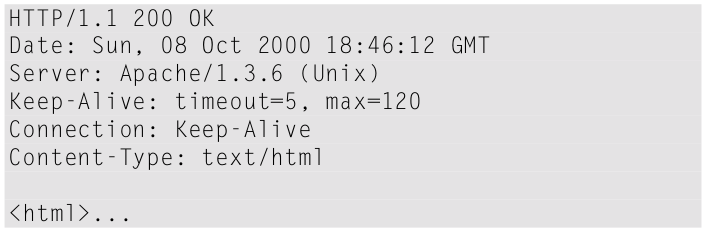
\includegraphics[width=0.6\textwidth]{images/ok.png} % Include the image placeholder.png
		\caption{OK message example}
	\end{center}
\end{figure}

%--------------------------
\section{Étude du Serveur Web Apache}
Apache est le serveur Web le plus populaire sur Internet. Plus que la majorité des sites Web sont basés sur elle. Ce qui rend Apache vulnérable à l'attaque qui sera analysée, c'est la manière dont il traite ses clients. En particulier, après avoir reçu une requête HTTP, un nouveau fil associé à cette conversation s'ouvrira. \\
Le serveur est fourni avec une variété de Modules Multi-Processus (MPMs) qui sont responsables de l'association aux ports réseau de la machine, acceptent les requêtes, et se chargent de répartir ces dernières entre les différents processus enfants. \\

%Les serveurs Apache plus anciens utilisent un modèle de limitation de thread, généralement un serveur Apache normal peut ouvrir environ 200 threads en parallèle. Normalement, la limitation n’est pas un problème pour les serveurs de site de petite taille, dans la mesure où ils n’ont pas besoin de gérer leur trafic.

\noindent
La table suivante fournit la liste des MPMs par défaut pour divers systèmes d'exploitation: \\

\begin{table}[H]
\begin{tabular}{|
>{\columncolor[HTML]{EFEFEF}}l |
>{\columncolor[HTML]{EFEFEF}}l |}
\hline
Netware & mpm\_netware                                                                                                  \\ \hline
OS/2    & mpmt\_os2                                                                                                     \\ \hline
Unix    & \begin{tabular}[c]{@{}l@{}}prefork, worker,\\ ou event, selon les possibilités de la plate-forme\end{tabular} \\ \hline
Windows & mpm\_winnt                                                                                                    \\ \hline
\end{tabular}
\end{table}

\noindent
Par exemple, pour un serveur Unix prenant en charge les threads multiples et les threads sécurisés avec interrogation, l'événement MPM sera utilisé. \\
Un processus de contrôle unique (le parent) a pour tâche de lancer les processus enfants. Chaque processus enfant crée un nombre fixe de threads serveurs selon la valeur de la directive ThreadsPerChild (25 par défaut), ainsi qu'un thread chargé d'attendre les connexions et de les passer à un thread serveur pour traitement au fur et à mesure de leur arrivée. \\
Le nombre maximum de clients pouvant être servis simultanément (c'est à dire le nombre global maximum de threads pour tous les processus) est défini par la directive MaxRequestWorkers (256 par défaut).


\subsection{Nginx vs Apache}
Nginx a été créé pour résoudre le problème de la gestion d’un grand nombre de connexions. Enfait, au lieu d’une architecture à base de threads, comme Apache, Nginx a une architecture pilotée par les événements qui ne crée pas de nouveau processus pour chaque requête. Dans notre projet, nous testerons l’attaque de slowloris sur différents serveurs Web et verrons si l’expérimentation

%--------------------------
\section{Étude du attaque Slowloris}
L'idée de base de l'attaque de slowloris est d'ouvrir de nombreuses connexions en envoyant des requêtes HTTP partielles. Des fractions de la demande sont envoyées ultérieurement à intervalles réguliers pour empêcher les sockets de se fermer. \\
This attack is different from other DoS attacks such as SYN flood attacks which misuse the TCP SYN (synchronization) segment during a TCP three-way-handshake. \\
On peut diviser un exploit suivant l'algorithme suivant: \\
\begin{itemize}
	\item On crée une requête GET destinée au serveur cible
	\item On envoie la requête byte par byte très lentement, dans l'ordre de secondes de delai
	\item On répète la même procédure avec un numero tres grand de messages, entre 100 et 200, dependant des configurations du serveur.
	\item Chaque GET répondu sera interprète dans le serveur comme un nouveau client; ça ouvre un nouveau thread dans le réservoir limité du serveur.
	\item Avec le temps, les requêtes lentes mais continues de la machine attaquante iront remplacer tous les connexions "légitimes".
\end{itemize}

\subsection{Slowloris detectability}
A desireble property of an attack is its non detectability. A Slow HTTP DoS attack is not commonly detected by Intrusion Detection Systems (IDS) since the attack does not contain any malformed requests. The HTTP request will seem legitimate to the IDS and will pass it onto the web server. Moreover the web servers logs will start to be presents only after the the requests are completed. This means that only when the attack has already got the server resources several hundred 400 errors will be presents in the logs. An interesting idea is to be developed is trying to set the timer between one fragment and onother in order to turn the error into 200 OK messages by completing a valid request.

%--------------------------
\section{Implémentation en Python}
Le travail d'implémentation a commencé en déterminant les aspects principaux requises. Fonctionnellement, nous avions
besoin d'un petit programme capable d’envoyer requêtes HTTP.Comme nous disons la section d'avant,
l'attaque \textit{slowloris} est fonctionnellement très élégant; en exploitant le mécanisme des GET
requests du protocole HTTP plusieurs fois, on occupe tous les \textit{threads} disponibles au serveur.
Alors, comme le but de notre état de l'art, on a fixé l'objectif d’implémenter un programme capable d'envoyer
GET requests à un serveur web HTTP.Cette fonctionnalité pourra après être déléguée à une fonction en python,
que l'on appellera lors de l'attaque dans une structure de contrôle plus intelligente.
Le but est d'utiliser les méthodes de Scapy, ce qui nous donnera la capacité de contrôler d'une façon plus granulaire
l'envoie des paquets. Le code source est travaillé et managé à travers de
git et le repositoire est disponible publiquement sur Github (documenté en anglais) sur le lien \href{https://github.com/AlessandroMontaldo/slowLorisAttack}{https://github.com/AlessandroMontaldo/slowLorisAttack}

\begin{lstlisting}
#!/usr/bin/env python
# Imports
from scapy.all import *
from scapy.all import http

# This handles HTTP responses from the server
def handle(pkt):
    if pkt.haslayer(http.HTTPRequest):
        print(pkt)
    
# Make a TCP SYN
#ip_address="35.204.58.85"    # Alessandro's server
ip_address="192.168.33.10"    # Matheus' VM (see Vagrantfile)
server_port=80                # http port
ip = IP(dst=ip_address)       # IP Packet 

# HTTP GET Request
get = "GET / HTTP/1.1\r\nHost: " + ip_address + "\r\n\r\n"
port = RandNum(1024,6500)

# The TCP 3-way handshake rules must be followed. As such, we begin by sending a
# TCP packet with the S (or SYN) flag set. The sequence number is irrelevant, as all
# future TCP packets will contain sequence numbers which are increments of the number
# given
SYN = ip/TCP(sport=port, dport=server_port, flags="S", seq=42) 

# Send SYN and wait for SYNACK as response
print(SYN.summary())
SYNACK = sr1(SYN)

# Send ACK and finally HTTP GET, sniff for the result
ACK=ip/TCP(sport=SYNACK.dport, dport=server_port, flags="A", seq=SYNACK.ack, ack=(SYNACK.seq+1))/get
sniff(filter="tcp and port 80", store=False, prn=handle)
\end{lstlisting}
%--------------------------
\section{Travaux futurs}
Le but des prochains travaux sera d'effectivement mettre une couche logique sur la méthode GET de tel façon
à obtenir le comportement attendu. Dans ce moment, la fonction principal du travail est http.py. La prochaine
étape sera de la transformer en une fonction qui reçoit un adresse IP et un numéro de porte. La logique d'allouer
numéro de portes sera toute faite par loris.py, que l'on développera à la suite. En termes de pseudo-code, on veut
à la fin que notre algorithme aie une logique (simplifiée) similaire à:


\begin{algorithm}
\caption{Une implémentation de slowloris}
\begin{algorithmic}

\STATE $target\_ip \leftarrow getIP()$
\FOR {( i=1,i $<=$ PORTS_{MAX}, i+)}
\END
\WHILE{1}
\STATE $target\_port \leftarrow randomNumber(1024,6554)$
\IF{isAvailable(target\_port)}
\STATE $incompleteGetRequest(target\_ip,target\_port)$
\ELSE

\ENDIF
%\WHILE{$N \neq 0$}
%\IF{$N$ is even}
%\STATE $X \leftarrow X \times X$
%\STATE $N \leftarrow N / 2$
%\ELSE[$N$ is odd]
%\STATE $y \leftarrow y \times X$
%\STATE $N \leftarrow N - 1$
%\ENDIF
%\ENDWHILE

\ENDWHILE
\end{algorithmic}
\end{algorithm}

\begin{thebibliography}{}
\bibitem{rfc}{Internet Engineering Task Force (IETF)\\
\href{https://tools.ietf.org/html/rfc1945}{Request for Comment 1945 - Hypertext Transfer Protocol 1.0}}

\bibitem{http-book}{THOMAS, Stephen \\
HTTP Essentials: Protocols for Secure, Scaleable Web Sites}

\bibitem{apache}{The Apache Group \\
\href{https://httpd.apache.org/docs/2.2/fr/new_features_2_0.html.fr}{Vue d'ensemble des nouvelles fonctionnalités d'Apache 2.0}}

\bibitem{apache-attacked}{Christian Folini, LWN.net group, archivé \\
\href{archive.wikiwix.com/cache/?url=http\%3A\%2F\%2Flwn.net\%2FArticles\%2F338407\%2FA}{Apache attacked by a slowloris}}

\bibitem{hackers}{Ha.ckers group, archivé \\
\href{https://web.archive.org/web/20150426090206/http://ha.ckers.org/slowloris}{Slowloris HTTP DoS}}

\bibitem{repo}{Repositoire Github \\
\href{https://github.com/llaera/slowloris.pl}{slowloris.pl, a perl implementation}}

\bibitem{repo}{Acunetix website \\
\href{https://www.acunetix.com/blog/articles/slow-http-dos-attacks-mitigate-apache-http-server/}{Acunetix blog - How To Mitigate Slow HTTP DoS Attacks in Apache HTTP Server}}

\end{thebibliography}

\end{document}
